\subsection{Интеграл с переменным верхним пределом. Теорема о непрерывности интеграла с переменным верхним пределом}

Рассмотрим функцию $f(t)$, которая интегрируема по Риману на отрезке $[a, b]$. Если мы зафиксируем нижний предел интегрирования $a$ и будем менять верхний предел $x$, то значение интеграла будет зависеть от $x$.

\subsubsection*{1. Определение}

\begin{definition}
Пусть $f \in R([a, b])$. Функция $\Phi(x)$, определенная на отрезке $[a, b]$ равенством:
\[ \Phi(x) = \int\limits_a^x f(t) dt, \quad x \in [a, b] \]
называется \textbf{интегралом с переменным верхним пределом}.
\end{definition}

Лектор отмечает, что такая функция часто встречается в физических задачах: если $f(t)$ — это скорость точки в момент времени $t$, то $\Phi(x)$ представляет собой перемещение точки за промежуток времени от $a$ до $x$.

\subsubsection*{2. Теорема о непрерывности}

Интегрируемость функции $f(x)$ гарантирует «хорошее» поведение функции $\Phi(x)$, даже если сама подынтегральная функция имеет разрывы (например, скачки).

\begin{theorem}
Если функция $f(t)$ интегрируема на отрезке $[a, b]$, то функция $\Phi(x) = \int_a^x f(t) dt$ является \textbf{непрерывной} на этом отрезке.
\end{theorem}

\begin{tcolorbox}[title=Доказательство, breakable]
Для доказательства непрерывности функции $\Phi(x)$ в произвольной точке $x \in [a, b]$ необходимо показать, что приращение функции $\Delta \Phi = \Phi(x + \Delta x) - \Phi(x)$ стремится к нулю при $\Delta x \to 0$.

1. Рассмотрим приращение функции $\Phi(x)$ в точке $x$:
\[ \Delta \Phi = \Phi(x + \Delta x) - \Phi(x) = \int\limits_a^{x + \Delta x} f(t) dt - \int\limits_a^x f(t) dt \]

2. Воспользуемся свойством аддитивности интеграла относительно отрезка интегрирования. Согласно этому свойству:
\[ \int\limits_a^{x + \Delta x} f(t) dt = \int\limits_a^x f(t) dt + \int\limits_x^{x + \Delta x} f(t) dt \]
Следовательно:
\[ \Delta \Phi = \int\limits_x^{x + \Delta x} f(t) dt \]

3. Так как функция $f(t)$ интегрируема по Риману на $[a, b]$, она обязана быть \textbf{ограниченной} на этом отрезке (необходимое условие интегрируемости). Значит, существует такое число $M > 0$, что для всех $t \in [a, b]$ выполняется:
\[ |f(t)| \le M \]

4. Оценим модуль приращения $\Delta \Phi$, используя свойство оценки интеграла через модуль и оценку интеграла через грань функции:
\[ |\Delta \Phi| = \left| \int\limits_x^{x + \Delta x} f(t) dt \right| \le \left| \int\limits_x^{x + \Delta x} |f(t)| dt \right| \]
Поскольку $|f(t)| \le M$, то:
\[ |\Delta \Phi| \le M \cdot |(x + \Delta x) - x| = M \cdot |\Delta x| \]

5. Из полученного неравенства $0 \le |\Delta \Phi| \le M |\Delta x|$ по теореме о зажатой функции (о двух милиционерах) следует, что:
\[ \lim_{\Delta x \to 0} \Delta \Phi = 0 \]
Это по определению означает, что функция $\Phi(x)$ непрерывна в точке $x$.
\end{tcolorbox}

\subsubsection*{3. Геометрический смысл}
Геометрически непрерывность функции $\Phi(x)$ означает, что при малом изменении верхнего предела $x$ на величину $\Delta x$, площадь криволинейной трапеции под графиком $f(t)$ меняется незначительно. Даже если функция $f(t)$ имеет скачок, «добавляемая» или «отрезаемая» узкая полоска шириной $\Delta x$ имеет площадь, стремящуюся к нулю, так как её высота (значение функции) ограничена.

\subsubsection*{4. Важное замечание}
Лектор подчеркивает, что из интегрируемости $f(x)$ следует только непрерывность $\Phi(x)$, но не её дифференцируемость. Для дифференцируемости интеграла с переменным верхним пределом потребуются более сильные условия на функцию $f(x)$, которые рассматриваются в следующем билете.

%\begin{center}
%\includegraphics[width=0.6\textwidth]{variable_limit_continuity.png}
% На чертеже изображен график ограниченной функции f(t), заштрихована 
% область под графиком от a до x (площадь Ф(x)) и выделена узкая 
% вертикальная полоска шириной Delta x, площадь которой соответствует 
% приращению Delta Ф.
%\end{center}

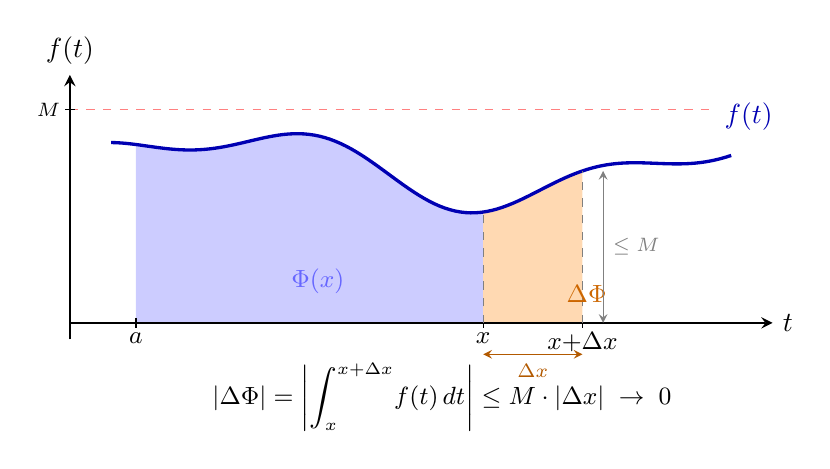
\begin{tikzpicture}[>=stealth, scale=1.05]
 
% ИСПРАВЛЕНО: #1 вместо \x
\pgfmathdeclarefunction{ff}{1}{%
  \pgfmathparse{0.4*sin(deg(#1*0.9))+1.9+0.2*cos(deg(2*#1))}%
}
 
\def\xa{0.8}
\def\xx{5.0}
\def\xdx{6.2}
 
% ИСПРАВЛЕНО: вычисляем координату середины полоски заранее
\pgfmathsetmacro{\xmidlabel}{(\xx+\xdx)/2+0.65}
\pgfmathsetmacro{\xmidarrow}{(\xx+\xdx)/2}
 
%--- Основная площадь Φ(x) ---
\fill[blue!20,domain=\xa:\xx,samples=80]
  plot(\x,{ff(\x)}) -- (\xx,0) -- (\xa,0) -- cycle;
 
%--- Полоска ΔΦ ---
\fill[orange!30,domain=\xx:\xdx,samples=40]
  plot(\x,{ff(\x)}) -- (\xdx,0) -- (\xx,0) -- cycle;
 
%--- Кривая ---
\draw[blue!70!black,very thick,domain=0.5:8.0,samples=120]
  plot(\x,{ff(\x)});
 
%--- Оси ---
\draw[->,thick] (0,0)--(8.5,0) node[right]{$t$};
\draw[->,thick] (0,-0.2)--(0,3.0) node[above]{$f(t)$};
 
%--- Метки ---
\foreach \xp/\lab in {\xa/{$a$},\xx/{$x$},\xdx/{$x{+}\Delta x$}}{
  \draw (\xp,0.06)--(\xp,-0.06);
  \node[below,font=\small] at (\xp,0) {\lab};
}
 
%--- Вертикали ---
\pgfmathsetmacro{\fx}{ff(\xx)}
\pgfmathsetmacro{\fxdx}{ff(\xdx)}
\draw[gray,dashed] (\xx,0)--(\xx,\fx);
\draw[gray,dashed] (\xdx,0)--(\xdx,\fxdx);
 
%--- Подписи площадей ---
\node[blue!60,font=\small] at (3.0,0.5){$\Phi(x)$};
% ИСПРАВЛЕНО: используем вычисленные координаты
\node[orange!80!black,font=\small] at (\xmidlabel,0.35){$\Delta\Phi$};
 
%--- Двойная стрелка ширины полоски ---
\draw[<->,orange!70!black,thin]
  (\xx,-0.38)--(\xdx,-0.38)
  node[midway,below,font=\scriptsize]{$\Delta x$};
 
%--- Оценка высоты ---
\draw[<->,gray,thin] (\xdx+0.25,0)--(\xdx+0.25,\fxdx)
  node[midway,right,font=\scriptsize]{$\le M$};
 
%--- Граница M ---
\draw[red!50,dashed,thin] (0,2.58)--(7.8,2.58);
\draw (0.06,2.58)--(-0.06,2.58);
\node[left,font=\scriptsize] at (0,2.58){$M$};
 
%--- Подпись ---
\node[font=\small] at (4.5,-0.9)
  {$|\Delta\Phi|=\left|\displaystyle\int_x^{x+\Delta x}\!f(t)\,dt\right|
    \le M\cdot|\Delta x|\;\to\;0$};
 
\node[blue!70!black,font=\itshape,right] at (7.8,2.5){$f(t)$};
 
\end{tikzpicture}
